\section{Udvikling og realisering af PCB}
Efter udvikling af de to versioner gennem simulering og testopstillinger, blev to PCB layout tegnet og produceret. Målet var at samle elektronikken på et PCB til at skabe stabilitet til microcontolleren og systemet som helhed. For at minimere størrelsen af printpladen og have så små strækninger for strømme og signaler som muligt, blev PCB'erne ikke ætset på universitet.
\\

Efter bestilling af PCB'erne blev der opdaget, at footprintet til microcontrolleren i den diskrete udgave var $7\milli\meter$ x  $7\milli\meter$, men den kan kun fås i $5\milli\meter$ x $5\milli\meter$.
\\

Det færdige PCB for den integrerede version kan ses på figur \ref{fig:PCB_IC} og \ref{fig:PCB_IC_bagside}, og den diskrete version ses på figur \ref{fig:PCB_diskret} og \ref{fig:PCB_diskret_bagside}.

\begin{figure}[h]
	\centering
	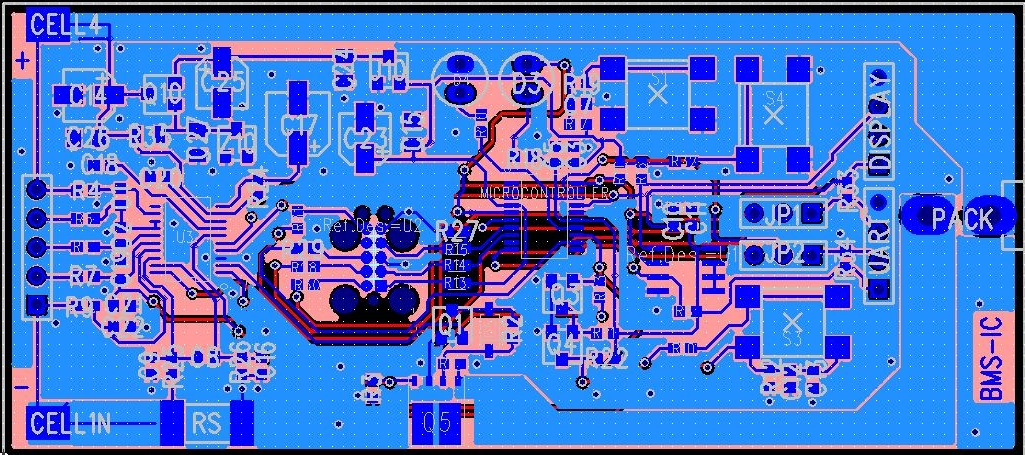
\includegraphics[width=15cm]{billeder/IC_1.jpg}
	\caption{Forsiden af PCB layout af BMS med batteriovervågningskreds.}
	\label{fig:PCB_IC}
\end{figure}

\begin{figure}[h]
	\centering
	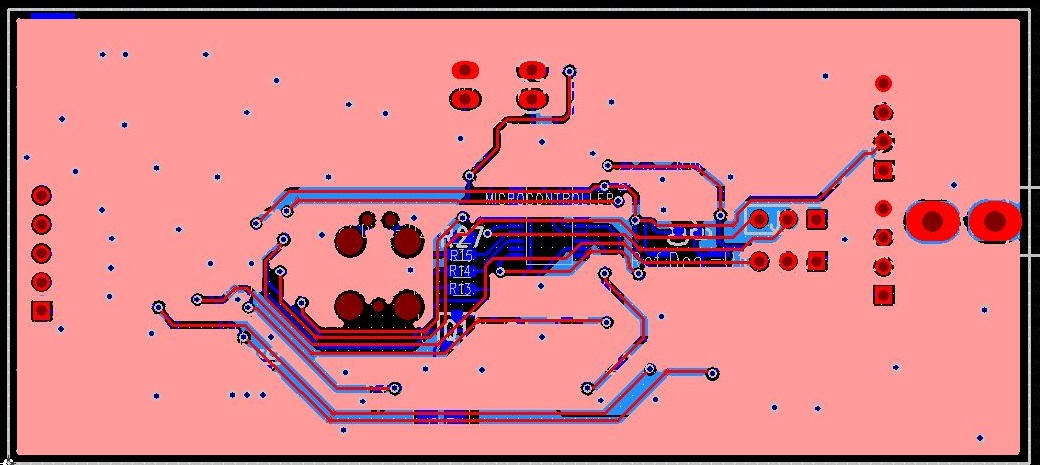
\includegraphics[width=15cm]{billeder/IC_2.jpg}
	\caption{Bagsiden af PCB layout af BMS med batteriovervågningskreds.}
	\label{fig:PCB_IC_bagside}
\end{figure}

\begin{figure}[h]
	\centering
	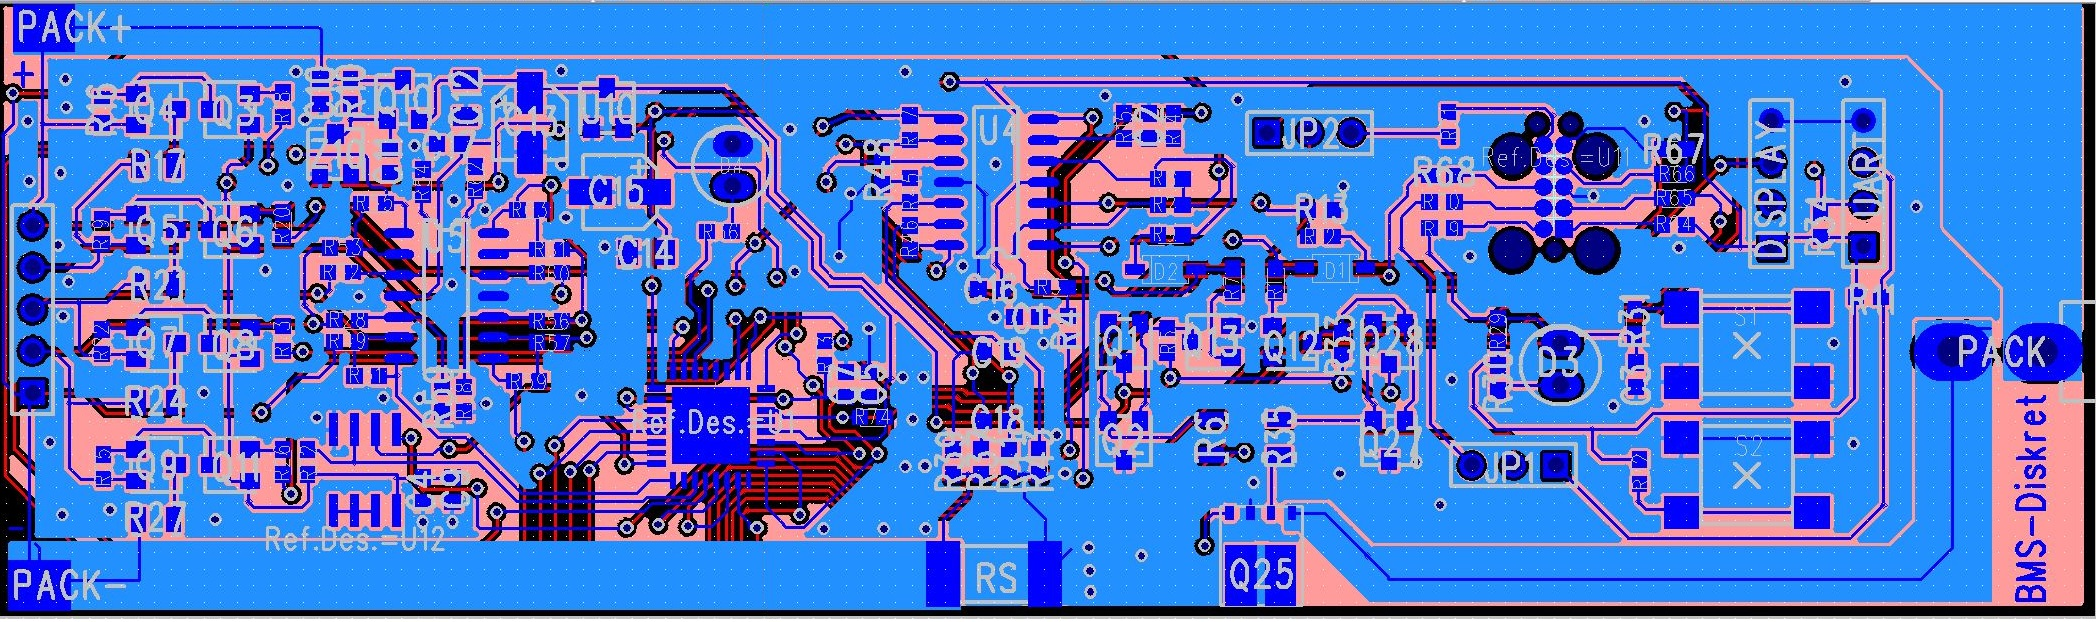
\includegraphics[width=15cm]{billeder/Diskret_1.jpg}
	\caption{Forsiden af PCB layout af diskret opbygget BMS.}
	\label{fig:PCB_diskret}
\end{figure}

\begin{figure}[h]
	\centering
	\includegraphics[width=15cm]{billeder/Diskret_3.jpg}
	\caption{Bagsiden af PCB layout af diskret opbygget BMS.}
	\label{fig:PCB_diskret_bagside}
\end{figure}